\documentclass[../report.tex]{subfiles}
\begin{document}
\onehalfspacing


\section{Read-Only Firmware}
% Because the RO Firmware is Read-Only, it is unable to updated during the life of the chromebook without dismantling the hardware.
% This is a double-edged sword for security purposes. 
% The RO FW is guaranteed to be the same code that shipped with the device, so one does not need to worry about it being compromised by attackers.
% However, any flaws in the shipped code are, by definition, unable to be patched and will remain a security vulnerability for the lifetime of the device.
% Because of these complications, the RO Firmware accomplishes the bare minimum of its responsibilities, leaving the more complicated tasks to the RW Firmware that is able to be patched ``In the Field''.

The Read-Only Firmware's purpose is to provide an initial configuration of the board's hardware and to verify the block of code that has been provided as the Read-Write Firmware.
The hardware required for this stage includes the TPM, SHA and RSA accelerator, and Flash.
If Developer Mode or Recovery Mode are enabled then the Keyboard, Display, and USB drivers will also need to be enabled.

The first thing that RO Firmware is responsible for is loading in all of the Flash memory to RAM so that it is more easily accessible. 
After Flash memory is in RAM, data structures like the GBB and the Firmware Image are populated by reading the flash map, which is always stored at a set location.
Once the data structures are populated and the hardware drivers are loaded, the Read-Only Firmware moves into the Vboot library to verify the next stage.

% RO FW destinations
The RO Vboot is responsible for checking the RW Vboot's validity and letting the RO Firmware whether it is safe to continue.
If the RO Vboot fails, there are many options it can decide to take.
Almost all of the RO Vboot failures leads to a ``recovery reason'' being stored in Flash and then power cycling the system.
If the system is booted with a recovery reason, the RO Firmware will take the Recovery path and request to be restored from a Recovery USB\@. %TODO: see early stages and giant stage image

\subsection{TPM Properties Used}

The RO Firmware is responsible for controlling the TPM setup and ensuring that its properties hold. 
The TPM is responsible for attesting the boot flags and protecting against rollback attacks. 
Setting the TPM up requires that the TPM is lead through its self-check, and that the data zones required by Chrome exist within the TPM's state.

% Physical Presence
% http://www.trustedcomputinggroup.org/wp-content/uploads/Physical-Presence-Interface_1-30_0-52.pdf pg 19
Chrome disables the physical protection in the RO Firmware.
Physical presence is something that can be set high or low on a TPM either through software commands or a hardware wire. 
If Physical Presence is set high, then the ownership of the TPM can be changed and the re-provisioning operations become available.
For this reason, Chrome completely disables this option by permanently locking the TPM to a low Physical Presence\@.

% Rollback Attack
% TODO: Rollback attack visual
The other thing that the TPM protects from is Rollback Attacks.
In this situation a rollback attack is when older software with known vulnerabilities replaces newer, protected software in a malicious ``upgrade''.
This attack works against a naive implementation because the attacker is relying on an older version of ChromeOS that is available, and unmodified.
Because the attacker is using Google's software, the software is signed by Google's private key and will be accepted by the VBoot algorithm.

\subsection{CBMC Verification}

\subsection{RO Firmware Properties}

The properties that we will be checking can be separated into 4 categories: array accesses, program flow, hyperproperties, and correctness.
The array access property restricts the writeable addresses in memory to valid array boundaries. 
Program flow properties refer to the execution path and function call stack throughout the program.
Correctness properties refer to facts about the code such that, if things were designed successfully, certain states shouldn't be reached.


\subsubsection{Memory Access Locations}

One of the things CBMC is used for most often is checking that array accesses are within bounds.
Array accesses are a problem in C programs because out of bound accesses allow buffer overrun attacks.
The following equation asserts that array accesses will always be within bounds.

\begin{equation}
    G(a \to (ptr + i < ptrHi(ptr) \land ptr + i < ptrHi(ptr)))
\end{equation}

This equation on its own is not strong enough for verified boot. 
Verified boot reads the image in as one contiguous blob and then uses size and offset variables to read more information.
CBMC is not able to detect that this pointer manipulation is an out of bounds array access so this must be manually checked with the following equation.

\begin{equation}
    G(a \to offset(struct) + size(struct) < size(img) \land offset(struct) + size(struct) > 0)
\end{equation}

Together these properties protect against buffer overruns occurring within the system.

\subsubsection{Program Flow properties}

\begin{figure}
  \centering
  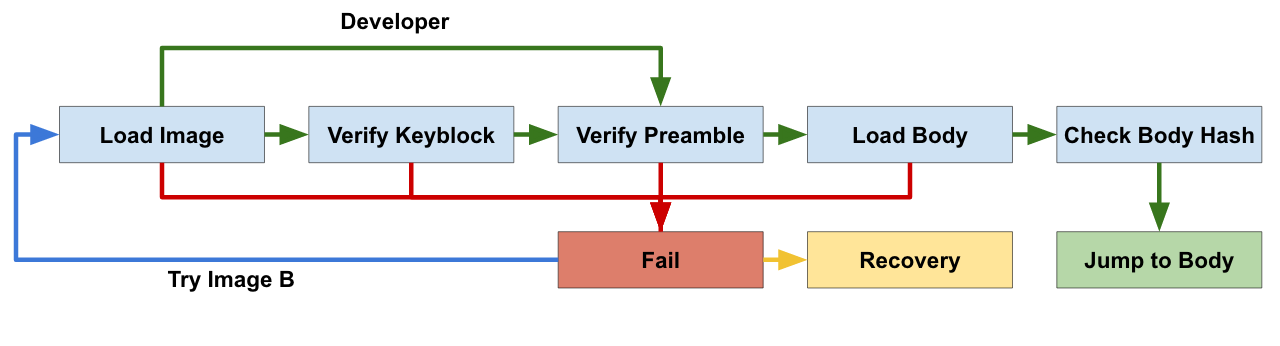
\includegraphics[width=0.8\linewidth]{verification_flow.png}
  \caption{The logical flow for verifying the firmware image}\label{fig:verif_flow}
\end{figure}

There needs to be an ordered constraint on the flow of the program. 
This constraint is responsible for checking that all stages of secure boot were called and in the correct order.
This will catch incorrect programs that skip steps or reading data that has not been verified yet.

Let $s_i$ correspond to the ith stage from Figure~\ref{fig:verif_flow}.

\begin{equation}
    G(s_0 \lor s_1 \lor s_2 \lor s_3 \lor s_4)
\end{equation}

\begin{equation}
    F(pass = F) \lor F(s_i \to s_{i+1})
\end{equation}

\begin{equation}
    G(s_i \to X(s_i \lor s_{i+1}))
\end{equation}

These equations state that the program must be in one of the 5 states, that each state can only transition to the next state, and that all state's except failure and the final state must transition eventually.

\subsubsection{Hyperproperties}

% TODO: Look at this later
% Verified boot contains many stages and each stage holds multiple flags and meta-data. 
% We want to make sure that untrusted information does not influence our booting sequence, be

\subsubsection{Correctness properties}

Verified boot allows for a number of different execution paths and can provide very different results depending on the system's state.
In order to prove that verified boot finished correctly, we can look at the following properties at the end of the boot sequence:

% Signature is correct when not in Dev mode
\begin{equation} \label{eq:sig_cor}
 \lnot M_d \land \lnot \text{verifySignature(img, rootKey)} \to XF (\text{pass} = F)
\end{equation}
% Hash is correct always 
\begin{equation} \label{eq:hash_cor}
    \text{hash(img.data)} \neq \text{img.hash} \to XF (\text{pass} = F)
\end{equation}
% Version should be greater than previously seen when not in recovery
\begin{equation} \label{eq:rollback}
    \lnot M_r \land (\text{img.version} < \text{prevVersion}) \to XF (\text{pass} = F)
\end{equation}

In the equations above, img is the image to be verified and rootKey is Google's public key loaded out of the GBB.
$M_d$ refers to developer mode being active and $M_r$ refers to recovery mode being active.
Img.version is the RW firmware version and prevVersion is the last seen version that is stored in the TPM\@.
Equation~\ref{eq:sig_cor} and Eq~\ref{eq:hash_cor} states that if the image's signature fails outside of Developer mode the whole boot will fail.
Equation~\ref{eq:hash_cor} states that if the image data's hash is not consistent with the hash stored in the image's metadata then the boot will fail.
Equation~\ref{eq:rollback} deals with the rollback assurance. It states that if the current version is lower than the last seen version (and we are not in recovery mode) then we will fail.

These properties will be proved contrapositively, meaning that when verified boot passes we will check that the antecedent is also false.

\subsubsection{Abstractions}

In order to get CBMC working, individual functions needed to be checked for properties at a time.
The full graph of functions can be seen at~\ref{fig:full_functions}.
While one function was being checked, the others were being used as abstracted functions.
In typical C fashion, each function has a return value which could be either success or an error code. 
Most functions could be abstracted to fail nondeterministically 

\begin{figure}
  \centering
  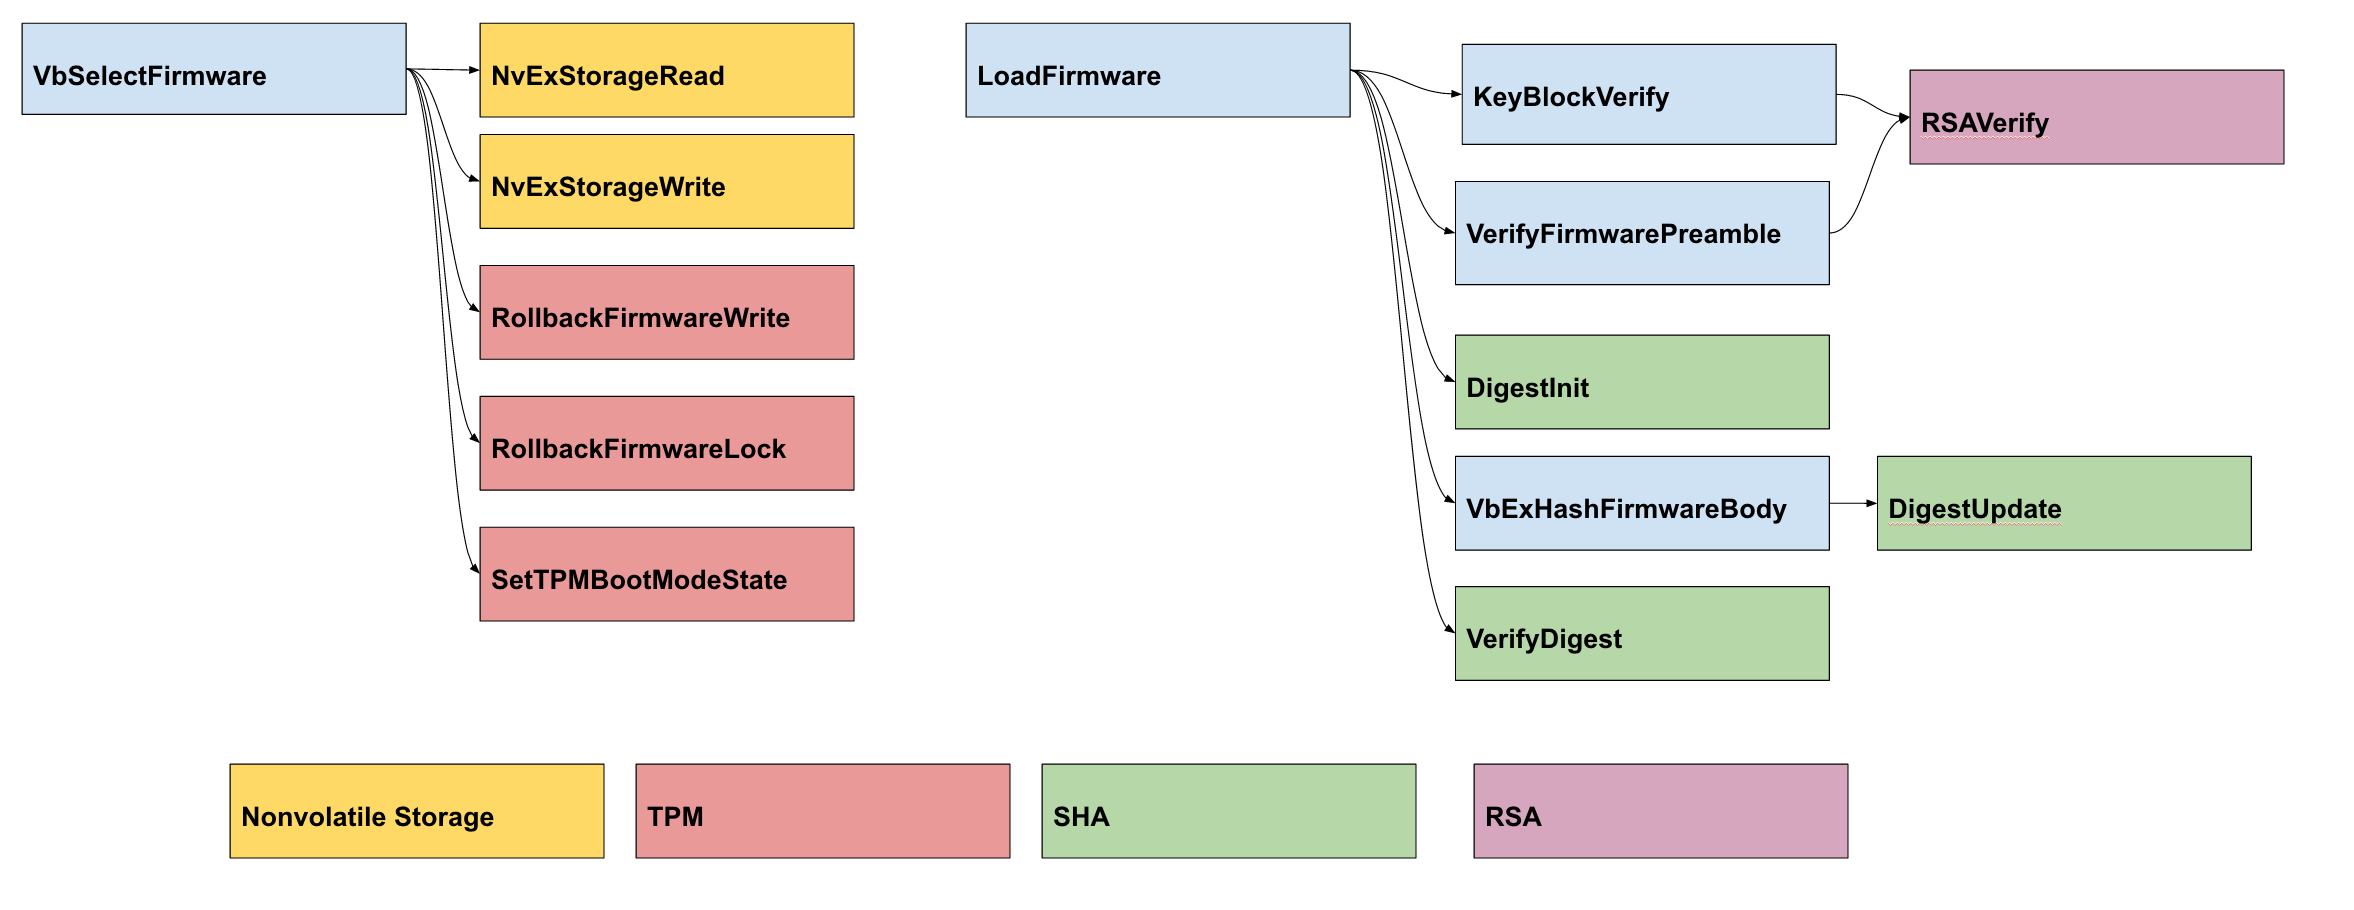
\includegraphics[width=0.8\linewidth]{ro_full_functions.png}
  \caption{The call graph of functions for Read Only Firmware}\label{fig:full_functions}
\end{figure}

\begin{table}[]
    \centering
    \caption{Results of CMBC tests run on Read Only Firmware}\label{cbmc_results}
    \begin{tabular}{|l|l|l|l|l|l|l|l|}
        \hline
        test name & steps & VCCs & vars  & clauses & time (s) & sat/unsat  \\ \hline \hline
        unit\_tests & 6554 & 39 & 1086730 & 24610811 & 14.59 & unsat \\ \hline
        rollback  & 4125 & 1 & 135239 & 1026823 & 4.79 & unsat \\ \hline
        rollback/dev & 4123 & 1 & 135276 & 1026983 & 4.68 & sat \\ \hline
        Image Failures & 4182 & 4 & 150593 & 1097362 & 4.45 & unsat \\ \hline
    \end{tabular}
\end{table}

\clearpage

\end{document}
